\documentclass[review]{elsarticle}

\usepackage[]{geometry}
\usepackage{amsmath}
\usepackage{tikz}
\usepackage[nomessages]{fp}
\usepackage{graphicx}
\usepackage{hyperref}
\usepackage{natbib}
\bibliographystyle{elsarticle-num}

\newcommand{\drawcirclerow}[5][0] { % args: [start], count, color, height, radius
  \FPadd\stop#2#1
  \foreach \i in {#1,...,\stop} {
    \ifnum \i < \stop
    \fill[#3] (\i, #4) circle (#5);
    \draw (\i, #4) circle (#5); 
    \fi
  }
}

\newcommand{\ra}{\rightarrow}
\newcommand{\sgcomment}[1]{\textcolor{red}{SG: #1}}


\journal{Theoretical Population Biology}

\begin{document}
\begin{frontmatter}
  \title{Counting parental contribution - how large sample size makes strong selection weak}

  \author{Ivan Krukov}
  \author{Simon Gravel}

  \begin{abstract}
    Neutral models of genetic diversity tend to be easier to analyze compared to models including
     selection. Because lineages are exchangeable in the neutral Wright-Fisher model, 
     for example, the number of lineages that are relevant to the ancestry of a sample at a single locus 
     can only decrease as we travel back in time.   
    As a consequence, useful recursion equations can be derived for patterns of polymorphism.  
    Under selection, by contrast, the number of relevant lineages can increase as we go back in time, 
    and the equivalent recursion equations do not close.
    Given a large enough sample size, however, the reduction in the number of lineages due to genetic drift 
    is larger than the increase in the number of lineages due to natural selection, and the number of relevant 
    lineages is unlikely to increase.
    We use this observation to derive asymptotically closed recursion equations for the distribution of 
    allele frequencies. 
    We show that this approach is accurate under strong drift and strong natural selection and ... 
    
    
    
     
    %In this work, we investigate the interplay of random genetic drift and selection in a finite
    %sample from a Wright-Fisher model. Normally, selection events increase the number of lineages
    %that contribute to a sample, so that the equations describing the time evolution of allele
    %frequencies in the sample are not closed. We show that by increasing the sample size, it is
    %possible to restore closure of the equations. With larger sample sizes, the number of coalescent
    %event increases, which compensates for the extra lineages required by selection. First, we
    %derive an exact Markov chain that describes the number of derived alleles in a sample, which we
    %use to calculate the allele frequency spectra under strong selection. Second, we investigate the
    %asymptotic properties of the process by studying the distribution of the number of contributing
    %lineages one generation into the past. We derive several approximations to inform when the
    %sample size is sufficiently large to overcome effects of selection.
  \end{abstract}
\end{frontmatter}

\section{Introduction}
\label{sec:introduciton}

The calculation of the site frequency spectrum (\textit{SFS}) is an important tool for the inference
of demographic histories and other population genetic parameters. In the absence of selection, the
number of parental lineages that contribute to the sample decreases back in time due to coalescent
events. This means that the equations are closed with respect to the sample size under neutrality.
This has paved the way for moment-based recursions of the allele frequencies
\cite{KimuraCrow1964,Ewens1972,DonnellyKurtz1999}. Recently, a number of successful methods,
including \cite{GutenkunstEtAl2009,JouganousEtAl2017,KammEtAl2017}, have become popular for this
purpose. At their core, these methods describe the time-evolution of the \textit{SFS}. The goal of
these approaches is to obtain the probability of observing a given number of derived alleles in a
finite sample conditional on the state of the parental lineages.

Despite many successes, considering selection has been problematic within this framework. Under
negative selection, the number of parental lineages that contribute to a sample can be larger that
the sample size itself, due to selective death events. As a consequence, the equation lose the
closure property \cite{JouganousEtAl2017}.

An extension to the Kingman's coalescent \cite{Kingman1982a}, the ancestral selection graph
(\textit{ASG}) \cite{KroneNeuhauser1997} considers the ancestry of a sample in the presence of
selection. The \textit{ASG} framework can be used to study the ancestry of highly deleterious
alleles \cite{Wakeley2009}, but it has not been used for inference, to our knowledge \sgcomment{I have not looked!}. Another
possible resolution is to use an uncontrolled jack-knife approximation to add extra lineages - the
method proposed in \cite{JouganousEtAl2017}.

Unlike the \textit{ASG}, the present treatment does not need to assume an infinitely large
population size, and also explicitly tracks multiple coalescent events, which is important with
large sample sizes \cite{BhaskarEtAl2014}. Our approach can be combined with the jackknife, but we
improve on it by deriving bounds on the performance our approximation.

\section{Background}
\label{sec:background}

First, consider the recursion describing the evolution of the \sgcomment{expected?} allele frequency spectrum
$\Phi_{n}^{(t)}$ in a sample of size $n$, without selection, where $t$ is the time in generations. There are two cases to be considered --
no coalescent event, where all \sgcomment{Watch out: there is no patental population of size $n$ -- this needs to be defined.} $p=n$ parental lineages contribute; and with a coalescent event,
where $p=n-1$ parental lineages contribute to the sample \sgcomment{You have not yet specified why you can assume a single coalescence}. Without a coalescent event, $p$ parental
lineages are sampled randomly into a present sample, so the allele frequencies remain the same:
$\Phi_{n}^{(t)}=\Phi_{n}^{(t-1)}$. With a single coalescent event, the contribution comes from $n-1$
parental lineages: $\Phi_{n}^{(t)}=\mathcal{D}(\Phi_{n-1}^{(t-1)})$, where $\mathcal{D}$ is a drift
operator\sgcomment{"a drift operator" is not a standard term I think -- we just came up with this in our paper. maybe "a n by n-1 sparse matrix"?}. Following the notation in \cite{JouganousEtAl2017}, we thus have:

\begin{align}
  \label{eq:op-neutral}
  \Phi_{n}^{(t)}=\Phi_{n}^{(t-1)}+\mathcal{D}(\Phi_{n-1}^{(t-1)})
\end{align}

In other words, the expected frequency spectrum of size $n$ at time $t$ can be obtained if only we know the expected frequency spectrum in a sample of identical size in the previous generation. This gives rise to a recursion formula for the frequency spectrum that can be solved efficiently\cite{JouganousEtAl2017}. Here we would like to generalize such an approach to cases including natural selection and large sample sizes.  


We first incorporate the effects of large sample size into our treatment. As previously shown in
\cite{BhaskarEtAl2014,NelsonEtAl2019}, the coalescent approximation may not be adequate in this
setting, since multiple coalescent events can take place within a single generation. With a slight
abuse of notation we denote $\mathcal{D}_i$ as the $i^{\text{th}}$-order diffusion event, which includes both
multiple (\textit{e.g.} several two-way) and multi-way (\textit{e.g.} four-way) coalescent. In
Appendix A, we demonstrate an efficient dynamic programming algorithm to exhaustively enumerate all
the events for a drift-only model.

With multiple coalescent, \eqref{eq:op-neutral} becomes:

\begin{align}
  \label{eq:op-neutral-mult}
  \Phi_{n}^{(t)}=\Phi_{n}^{(t-1)}+\sum_{i=1}^{n}\mathcal{D}_i(\Phi_{n-i}^{(t-1)})
\end{align}

The equation \eqref{eq:op-neutral-mult} is still closed in terms of the sample size, since
$\Phi_{n}^{t}$ only depends on $p=(n-i)<n$ parental lineages. However, if we consider
selective death events, the number of contributing parental lineages increases back in time. For
example, in case of a single selective death event, we have
$\Phi_{n}^{(t)}=\mathcal{S}(\Phi_{n+1}^{(t-1)})$, with selection operator $\mathcal{S}$. Multiple
selection events are possible per generation, but we restrict our attention to the case where each
lineage experiences at most one selective death event. This still allows us to consider strong
selection, with at most $p<=2n$ parental lineages contributing: \sgcomment{Where did the drift + selection terms go?}

\begin{align}
  \label{eq:op-selection}
  \Phi_{n}^{(t)}=\Phi_{n}^{(t-1)}+\sum_{i=1}^{n}\mathcal{D}_i(\Phi_{n-i}^{(t-1)}) + \sum_{j=0}^{2n}\mathcal{S}_j(\Phi_{n+j}^{(t-1)})
\end{align}

The closure no longer holds for \eqref{eq:op-selection}, as up to $2n$ parental lineages can
contribute to the sample. However, as we will show throughout this work, increasing sample size $n$
restores closure asymptotically. This is can be seen from the context of the \textit{ASG}. The
number of (parental) lineages $p$ in the graph can be described as a birth-death process
\cite{KroneNeuhauser1997, Wakeley2009}:

\begin{align}
  \label{eq:asg-size}
  p \ra \begin{cases}
      p+1 & \text{at rate } Nsp  \text{ (selection) }\\
      p-1 & \text{at rate } p (p-1)/2 \text{ (coalescent) }
    \end{cases}
\end{align}

The death rates of the parental lineages due to coalescence is of the order of $p^2$, while the
birth rate due to selection events is of the order of $Nsp$. Thus, drift will dominate the process in
the cases where $Ns < p$. \sgcomment{I'm a bit confused about why the population size $N$ made its way in equation 4. I think this is because you are reporting things in "coalescent time" units. I would recommend using physical units, since this way you don't have to go back and forth.  }

The rest of the paper is organized into two sections. In the first section, we construct a Markov
process to track the number of derived lineages in a large sample from a Wright-Fisher model,
similar to \cite{JouganousEtAl2017,KammEtAl2017}. In this, we fully account for multiple coalescent
events per generation, and show that we restore closure with increasing sample size. In the second
part, we derive a number of asymptotic results to get a better understanding of the process. We
construct an exact probability distribution for the number of contributing parental lineages,
together with several approximations. Importantly, we derive a normal approximation that allows us
to calculate a quantile of the sample size where the system is approximately closed.

\section{Results}
\label{sec:results}

\subsection{Markov process construction}
\label{subsec:markov}

We seek to construct the process that describes the time evolution of the derived allele count in a
sample of size $n$, from a Wright-Fisher population of size $N$. Here, we consider a haploid model,
but the results should hold approximately with the correction to the population size. The goal is to
construct a probability of going from $i$ to $j$ derived alleles in a sample of size $n$, which we
denote as $(j,n)\ra(i,n)$.

Under neutrality, the knowledge of the parental configuration is sufficient to construct the
transition probabilities. Since we want to account for multiple coalescent events, parental
configurations of sizes $p \in [1, n-1]$ can all contribute \eqref{eq:op-neutral-mult}. For example,
$n-2$ parental lineages will contribute if there if a single coalescence of four lineages, or double
coalescence of two lineages. The number of contributions increases rapidly.

If we want to consider every possibility, it is useful to use a dynamic programming approach where
we construct every transition probability matrix in for the (parental) sample sizes $p \in [1,n-1]$.
Then the transition probabilities $P((j,n)\ra(i,n))$ can be obtained from $P((j,n-1)\ra(i,n-1))$.
We derive this equation in appendix A.

In the case with selection, the number of parental lineages $p$ can exceed $n$: $p\in[1, \infty]$.
We restrict our attention to the cases where parents of each lineage in the sample experience at
most one selective death event (\textit{i.e.} $s \ll 1$), so we consider the range of $p \in [1, 2n]$.
However, we can still consider cases where $ns > 1$.

We therefore want to find $Q((j,m)\ra(i,n))$ (note that the current and parental sample sizes, $n$
and $m$ can be different) in terms of $Q((j',m')\ra(i',n-1))$, where $m' \in [1, 2n]$, $j',i' \in
[1, m']$. The list of events that contribute to $Q((j,m)\ra(i,n))$ is shown in Figure
\ref{fig:recurrence}, and the full derivation is in appendix B.

\begin{figure}
  \centering
  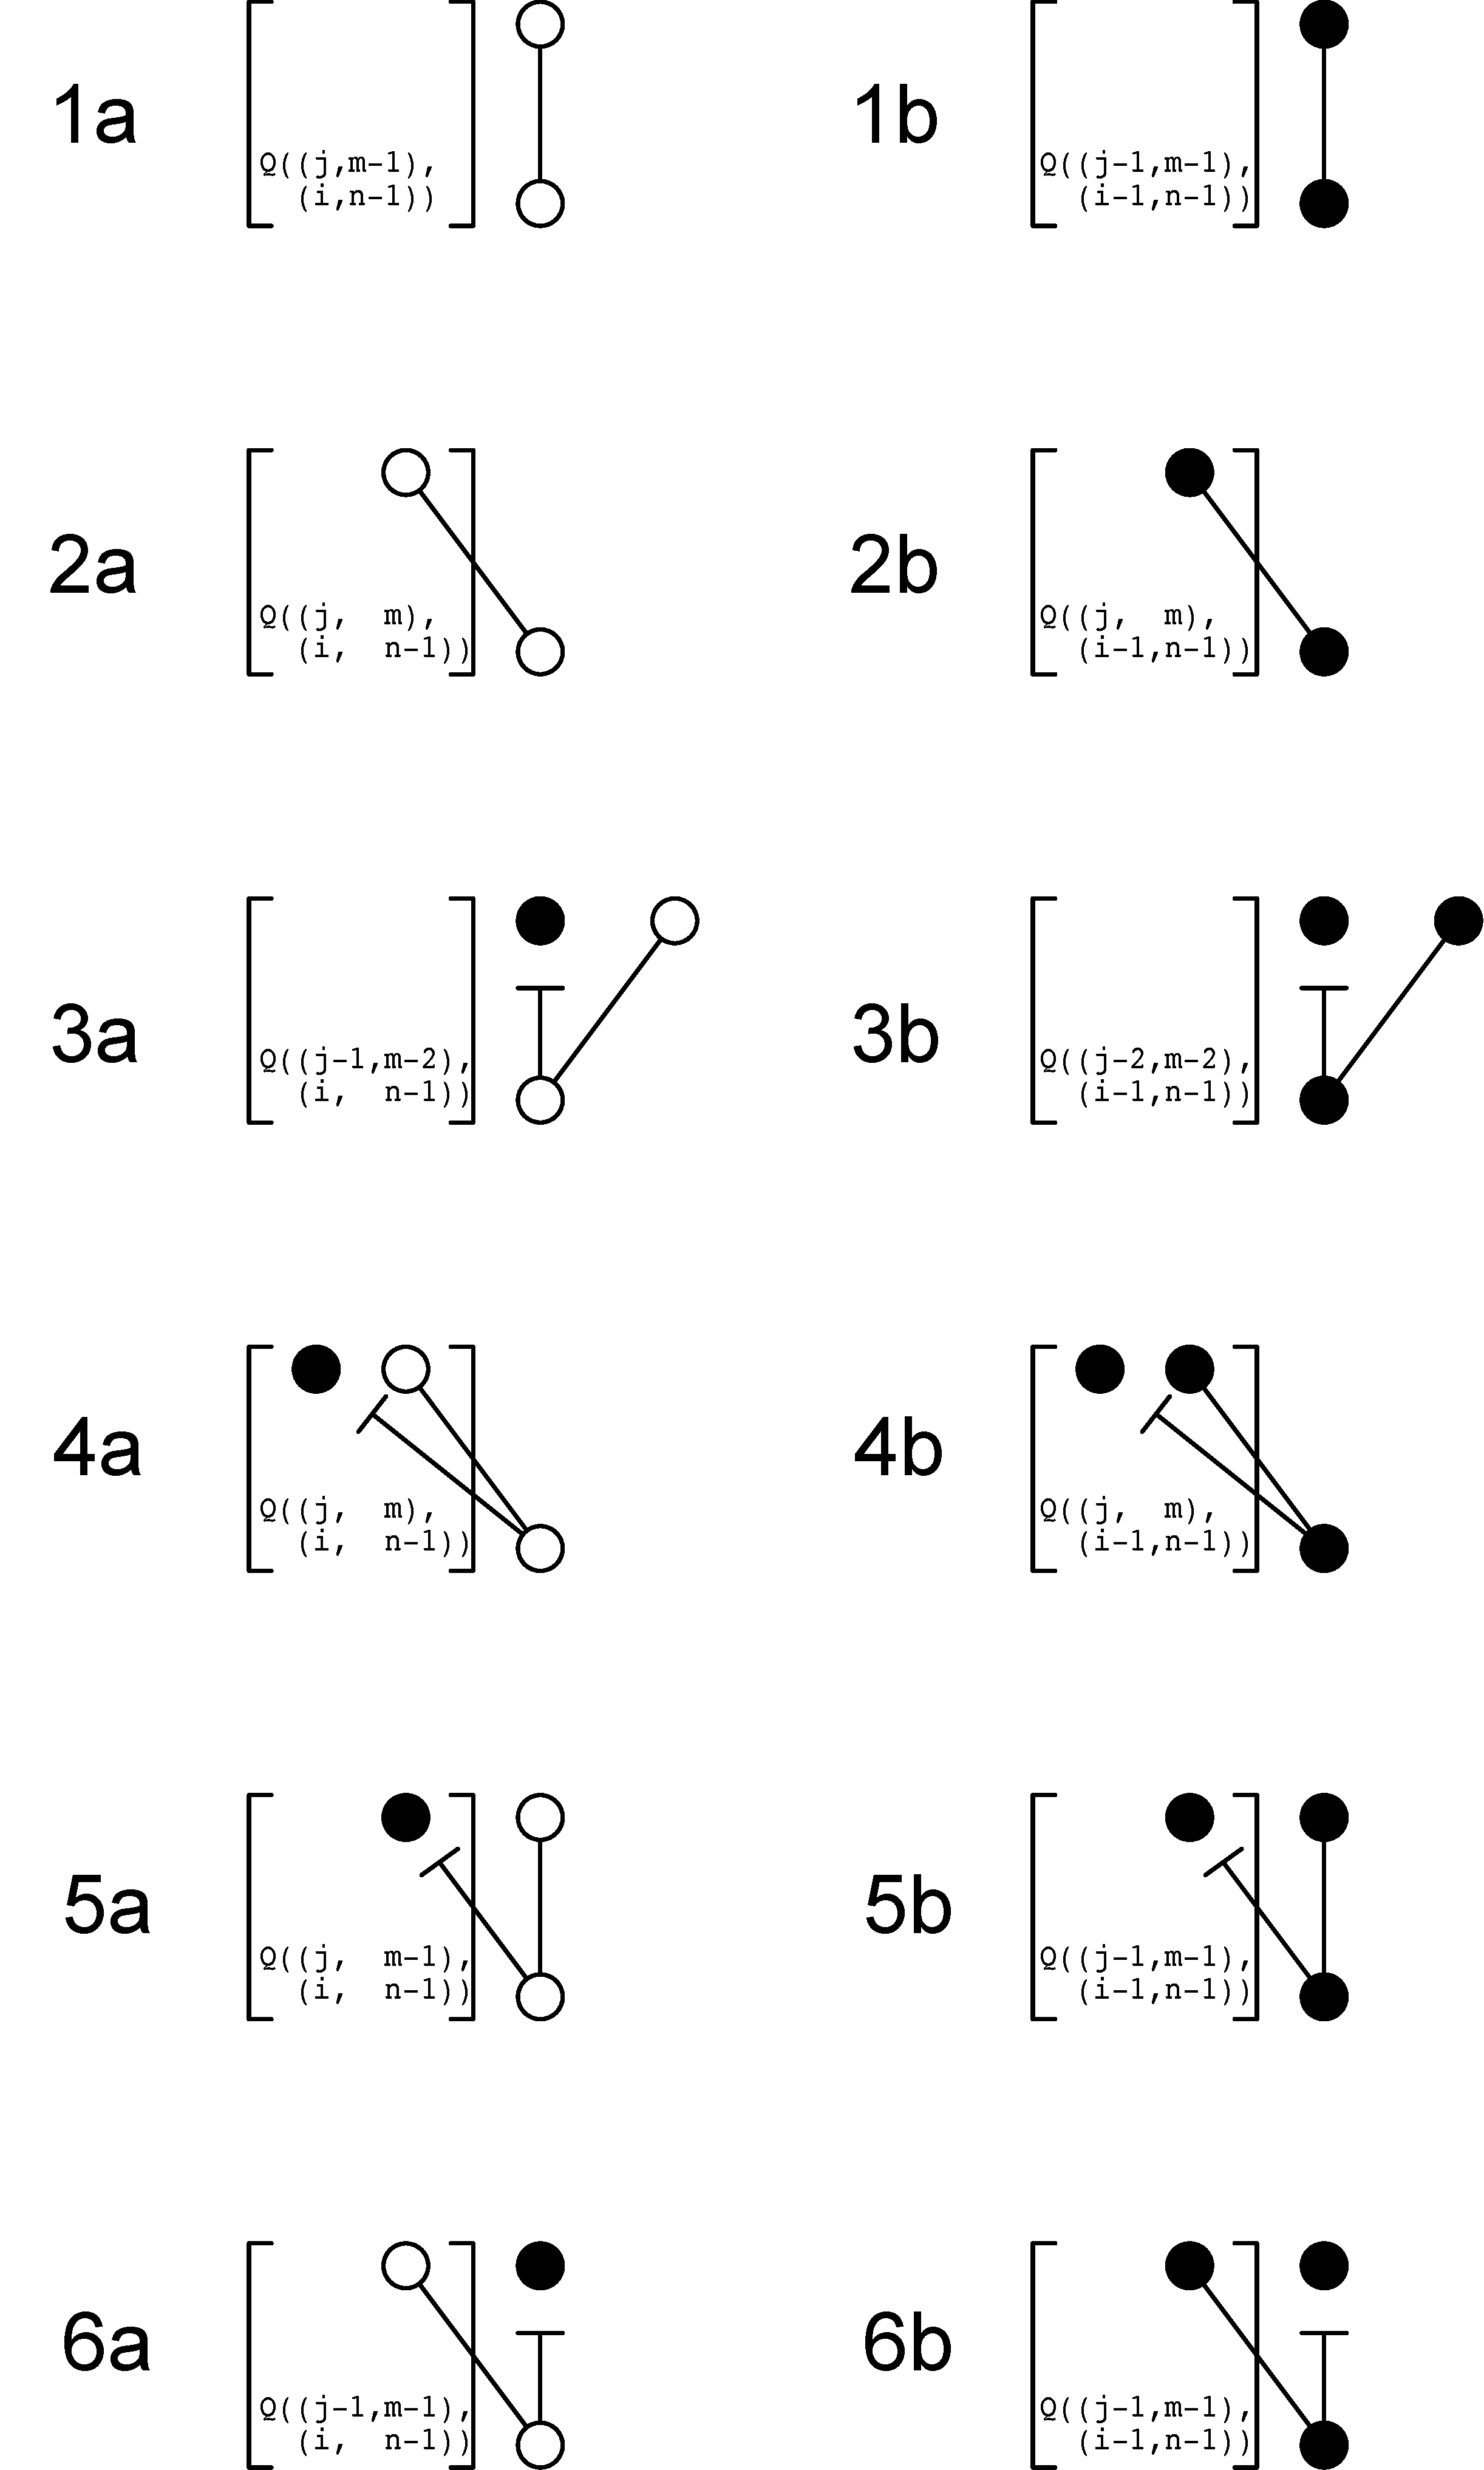
\includegraphics[height=0.7\textheight]{fig/recurrence.pdf}
  \caption{Contribution of parental configurations to a present sample. The transition probability
    at $Q((j,m)\ra(i,n))$ is the sum of 12 terms shown in the figure. The filled circles indicate
    derived alleles, empty circles - ancestral alleles, lines show ancestral descent. The square
    brackets and the align within indicate the parental configuration that contributes to the
    entry. Full derivation is shown in appendix B.}
  \label{fig:recurrence}
\end{figure}

In addition to every transition probability matrix of size $p \in [1, n-1]$, the calculation in the
case with selection additionally requires the calculation of rectangular matrices where the number
of parental contributors ($p' \in [1, 2n]$) is not equal to the sample size. As a result, the
calculation time is of the order of $O(n^4)$ for the selection case, while it is only $O(n^3)$ for
the neutral case.

\subsection{Calculation of site frequency spectra}
\label{subsec:afs}

Once the matrix $Q$ is constructed, it can be used to calculate the site frequency spectrum within a
sample. For the infinite sites model at equilibrium, we can calculate the \textit{SFS} $\Phi$ as a
solution to a linear system:

\begin{equation}
  \label{eq:sfs-calc}
\Phi = \Phi Q + n \mu e_1
\end{equation}

where $\mu$ is the per-site mutation rate, and $e_1$ is the first column of the identity matrix of
size $n$. Figure \ref{fig:strong-selection} shows the comparison of the \textit{AFS} calculated from
\eqref{eq:sfs-calc}, the diffusion approximation \cite[eq. 9.23]{Ewens2004}, and the calculation
performed in \texttt{Moments} \cite{JouganousEtAl2017}. Panel A shows a comparison at $Ns=100$, with
the population size ($N=2000$), which is substantially larger than the sample size ($n=200$). There
is a small deviation between the approaches at large allele frequencies. However, since highly
deleterious alleles are unlikely to reach these frequencies, the difference is immaterial. At
stronger selection coefficients, \texttt{Moments} suffers from numerical instability, while the
diffusion approximation performs well (not shown).

If the sample size is the same as the population size ($n=N=200$) (Fig.
\ref{fig:strong-selection}B), the diffusion approximation and \texttt{Moments} perform poorly, while
our approach remains stable. This is expected, since the diffusion framework does not perform well
if multiple coalescent events contribute.

\begin{figure}
  \centering
  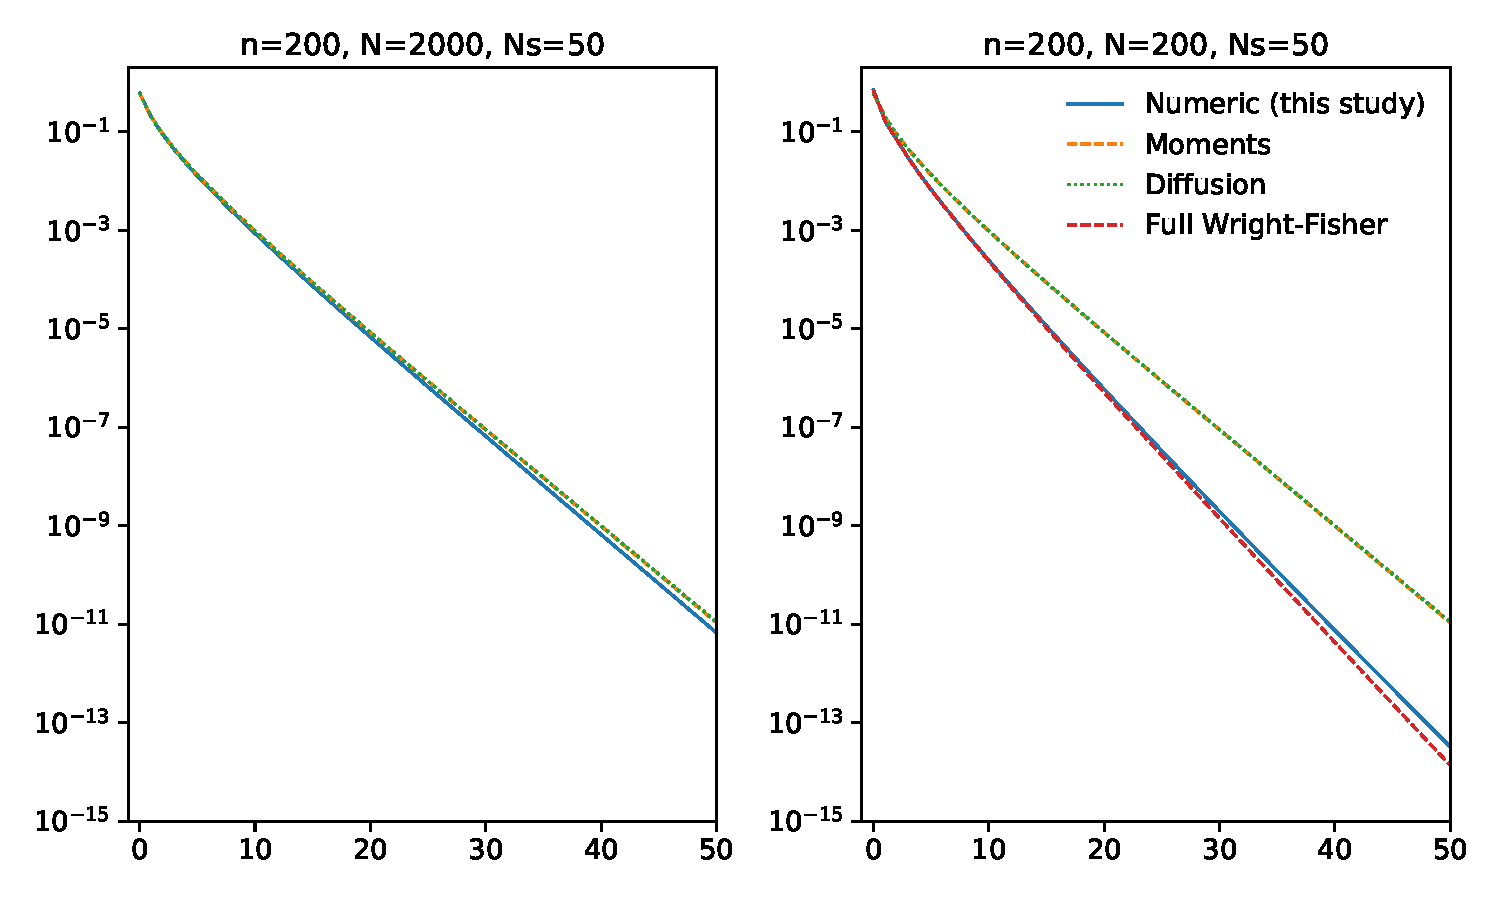
\includegraphics[width=0.7\textheight]{fig/strong_selection.pdf}
  \caption{Site frequency spectra in a sample of size $n=200$, for highly deleterious alleles
    ($Ns=-50$). (A) shows the frequency spectrum in a sample from a large population ($N=2000$), (B)
  in a small population ($N=200$). Both panels are truncated at $10^{-15}$, to show only
  sufficiently high allele frequencies. Y-axis on a logarithmic scale.}
  \label{fig:strong-selection}
\end{figure}

\subsection{Closure properties}
\label{subsec:closure}

To show the closure properties of $Q$, we can calculate the total probability that more that $n$
parental lineages contribute to the sample of a given size. By construction, the sum of rows of $Q$
should correspond to the total probability mass that included configurations contribute
(Fig. \ref{fig:recurrence}). Thus, the probability that some number of configurations are
unaccounted for, with $j$ derived alleles in the sample, is given by
$1-\sum_{i=0}^{n}Q_{i,j}$. Figure \ref{fig:missing} shows the probability of missing configurations
in a sample size of $n=200$, for $j=200$ derived lineages.

\begin{figure}
  \centering
  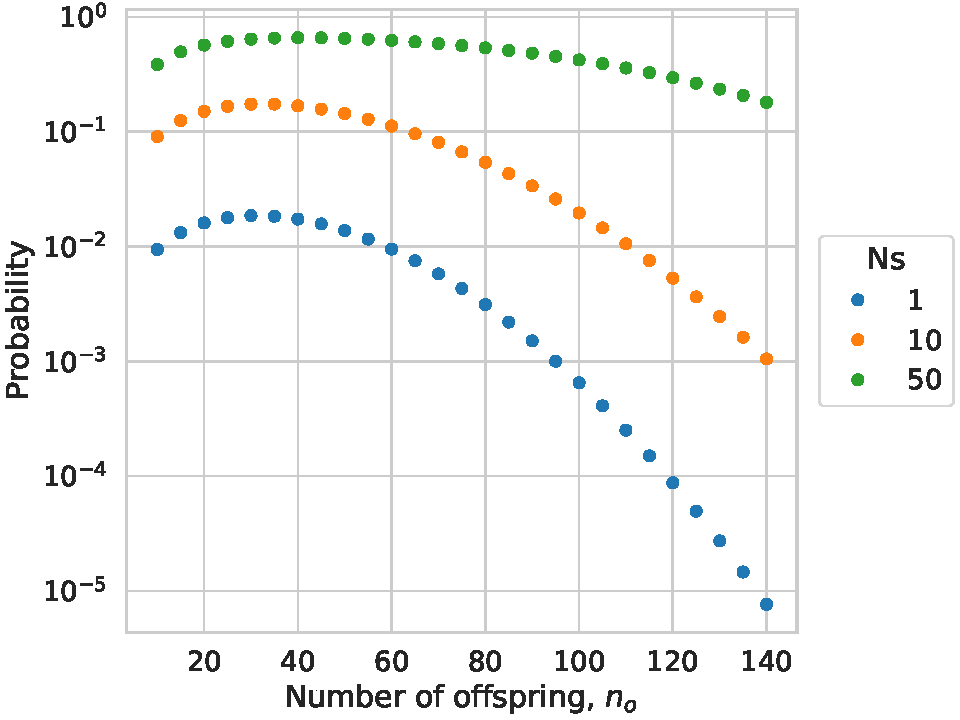
\includegraphics[]{fig/missing.pdf}
  \caption{Probability that unaccounted lineages contribute to the transition probabilities. The
    probabilities are calculated as 1 minus the sum of probabilities for the state where every
    allele is derived.}
    \label{fig:missing}
\end{figure}

It is evident that above some threshold, the number of missing lineages becomes negligible, but it
is not clear where that threshold is. Intuitively, the increasing sample size should increase the
number of drift events quadratically, while the number of selection events scales linearly with the
sample size \eqref{eq:asg-size}. In the next section we investigate the necessary sample size that
ascertains that all (or most) contributing lineages are accounted for.

\section{Asymptotic closure properties}

We now want to determine what sample size is sufficient so that the number of coalescent events due
to drift is larger than the number of selection events, such that the system remains closed
\eqref{eq:op-selection}. We derive several approximations to the model proposed in the first
section,in order to get a better understanding of this behavior.

As a first order approximation, we consider the mean number of lineages that contribute via the two
processes. Then, we construct a full probability distribution of the number of contributing lineages
one generations into the past. Finally, we propose a normal approximation to this distribution, in
order to derive a simple quantile function for the number of used lineages.

Consider the behavior of a single biallelic locus in a haploid Wright-Fisher model with a population
of size $N$. We consider a sample of size $n$ from within the population, where $n$ is not
necessarily much smaller than $N$. We want to know how many parents $p$ have contributed to the
present sample from one generation in the past. We first derive a distribution that provides an
upper bound.

\begin{figure}
  \centering
    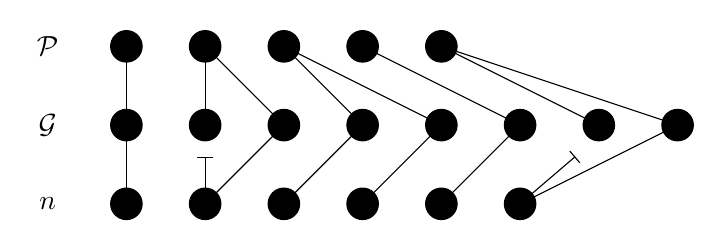
\begin{tikzpicture}
      \node at  (0, 0) {$n$};
      \node at  (0, 1) {$\mathcal{G}$};
      \node at  (0, 2) {$\mathcal{P}$};
      % 
      \draw     (1, 0) -- (1, 1);
      \draw[-|] (2, 0) -- (2, 0.6);
      \draw     (2, 0) -- (3, 1);
      \draw     (3, 0) -- (4, 1);
      \draw     (4, 0) -- (5, 1);
      \draw     (5, 0) -- (6, 1);
      \draw[-|] (6, 0) -- (6.7, 0.6);
      \draw     (6, 0) -- (8, 1);
      %
      \draw     (1, 1) -- (1, 2);
      \draw     (2, 1) -- (2, 2);
      \draw     (3, 1) -- (2, 2);
      \draw     (4, 1) -- (3, 2);
      \draw     (5, 1) -- (3, 2);
      \draw     (6, 1) -- (4, 2);
      \draw     (7, 1) -- (5, 2);
      \draw     (8, 1) -- (5, 2);
      %
      \drawcirclerow[1]{5}{black}{2}{0.2} % parents
      \drawcirclerow[1]{8}{black}{1}{0.2} % intermediate
      \drawcirclerow[1]{6}{black}{0}{0.2} % offspring
    \end{tikzpicture}  
    \caption{Sampling scheme to produce a sample of size $n$. Every generation a random number of
      $\mathcal{P}=p$ parents (of which a fraction $x$ is derived), produce a large number of
      gametes $\mathcal{G}=g$. To form the sample, $n$ individuals pick from the gamete pool. With
      probability $xs$, picking a gamete fails, and a new gamete is drawn from the pool.}
    \label{fig:sampling}
\end{figure}

Each generation, a random number of $\mathcal{P}=p$ individuals (parents) produce a large random
number of gametes, $\mathcal{G}=g$ - Figure \ref{fig:sampling}. Then we form $n$ individuals in the present
generation by randomly sampling gametes, without replacement. The probability of a successful sample
for a particular individual is $1-xs$, where $x$ is the frequency of the derived allele in the
parental generation. Then with probability $xs$, a new gamete is drawn from the pool. This sampling
scheme allows us to consider drift ($p \rightarrow g$) and selection ($g \rightarrow n$) as distinct
processes.

We want to know the upper bound on the number of lineages used. Since the maximum number of lineages
will be resampled when all lineages are derived, we will usually assume $x=1$ in the following
calculations. This also allows to treat the lineages as exchangeable \cite{Wakeley2009}. Note that
in section \ref{subsec:markov}, we did not assume exchangeability of lineages, which led to a
considerably more complex formulation.

For a given sample size, the probability that $p$ parents have contributed is:

\begin{align}
  \label{eq:conditional}
  Pr(\mathcal{P}=p|n) = \sum_{\mathcal{P}}Pr(\mathcal{P}=p|\mathcal{G}=g)Pr(\mathcal{G}=g|n)
\end{align}

Where $\mathcal{P}$ and $\mathcal{G}$ are random variables denoting the number of contributing
parents and gametes, respectively.

Before deriving the distribution formally, we seek to obtain several approximate results.

\subsection{Expected number of lineages used}
\label{subsec:exp-number}

First, we seek an approximate expression for the expectation of the total number of lineages used.
This can be approximated as the sum of expectations of the number of lineages sampled under drift
plus the number of lineages rejected by selection (selective deaths). The number of parents that
contribute to $n$ gametes (drift) will be:

\begin{align}
  \hat{E}[\mathcal{P}|n] = N(1-\left( 1 - \frac{1}{N} \right)^n)
\end{align}

The probability of selecting a particular parent is $\frac{1}{N}$, so the probability of selecting
different parents for $n$ individuals is $(1-\frac{1}{N})^n$. Then one minus this value is the
probability that the same parent was picked at least once by any of the $n$ individuals.

For selection, we want to consider the expected number of gametes that are rejected by selection
to form a sample size of $n$. If the probability of rejection is $xs$, the scheme is described by the
negative binomial distribution, where the random variable is the number of failures, given $n$
successes. The expectation of this parameterization of negative binomial is:

\begin{align}
  \label{eq:neg-binom-fail}
  \hat{E}[\mathcal{G}-n|n] = n\left( \frac{xs}{1-xs}\right)
\end{align}

Then summing the expectations of the two random variables yields:

\begin{align}
  \hat{E}[\mathcal{P}+\mathcal{G}-n] &= \hat{E}[\mathcal{G}-n|n] + \hat{E}[\mathcal{P}|n] \\
  &= N(1-\left( 1 - \frac{1}{N} \right)^n) + n\left( \frac{xs}{1-xs}\right) \\
  &\underset{N\gg n}{\approx} \frac{nxs}{1-xs} - \frac{n^2}{2N}
\end{align}

The second approximation is made under the assumption that the sample size is much smaller than the
population size. We can see that the expected number of lineages sampled will be increased by
selection as a linear term. Drift tends to decrease the number of lineages as a quadratic term with
respect to the sample size. This is analogous to the results from the ancestral selection graph
\cite{KroneNeuhauser1997}, but now includes sample size directly.

We now want to ask when the expected number of lineages is less that the sample size:

\begin{align}
  \label{eq:critical-sample}
  \hat{E}[\mathcal{P}] &< n \nonumber \\
  \frac{nxs}{1-xs} - \frac{n^2}{2N} &< n \\
  n &\ge \frac{2Nxs}{1-xs} \nonumber \\
  &\approx 2Nxs
\end{align}

This allows us to derive a simple expression for the sample size where drift overcomes selection.
Figure \ref{fig:critical-sample-size} shows this for several selection coefficients, assuming the entirety
of the sample is derived in a population of $N=1,000$. The $Y$ axis shows the fraction of
contributing parental lineages to the sample size, $\frac{p}{n}$. Above the horizontal line
$\frac{p}{n} > 1$, selection dominates. Below, drift reduces the number of used lineages. The
intercept of the line with $\frac{p}{n} = 1$ is the critical sample size, which is
well-approximated by $2Ns$.

\begin{figure}
  \centering
  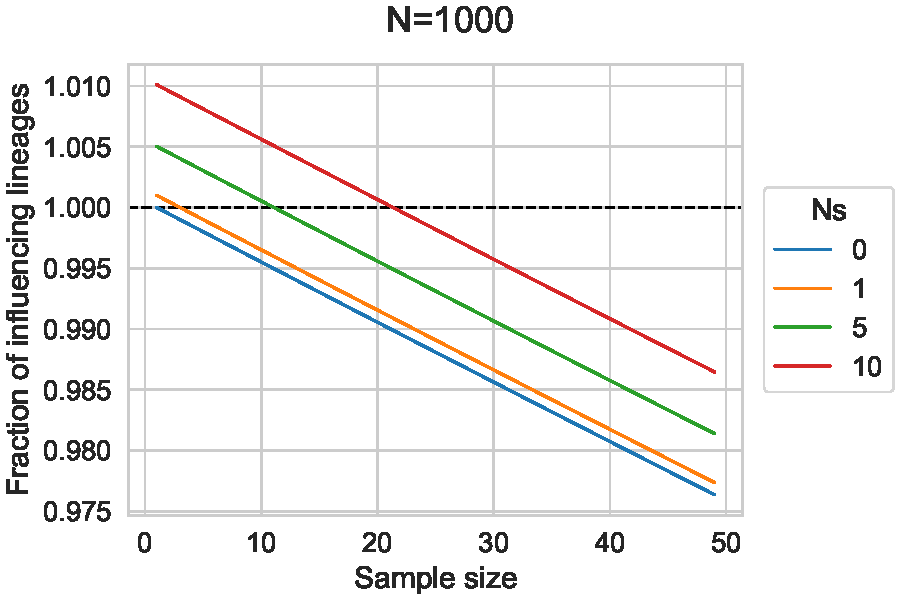
\includegraphics{fig/critical_sample_size.pdf}
  \caption{Critical sample size for different selection coefficients. The $Y$ axis shows the
    fraction of parental lineages over the sample size, $\frac{p}{n}$, each line corresponds to a
    different selection coefficient. Above $\frac{p}{n}\ge 1$, selection dominates, below -- drift.
    The critical sample size, where the expected number of parental contributing lineages is smaller
    than the sample size is well-approximated by $2Ns$.}
  \label{fig:critical-sample-size}
\end{figure}


Using the same equation, we can track the expected number of used parental lineages back in time,
which we denote as $n_{t-1}$:

\begin{align}
  \label{eq:contributors-back}
  n_{t-1}=\frac{n_txs}{1-xs} - \frac{n_t^2}{2N}
\end{align}

We solve this recurrence going back in time 10,000 generations, producing figure
\ref{fig:bell-plot}. The equilibrium point is well-approximated by $2Ns$, shown as a dashed line
here. This is the same as solving equation \ref{eq:critical-sample} explicitly. Non-withstanding of
the starting sample size, we converge to the equilibrium relatively quickly.

\begin{figure}
  \centering
  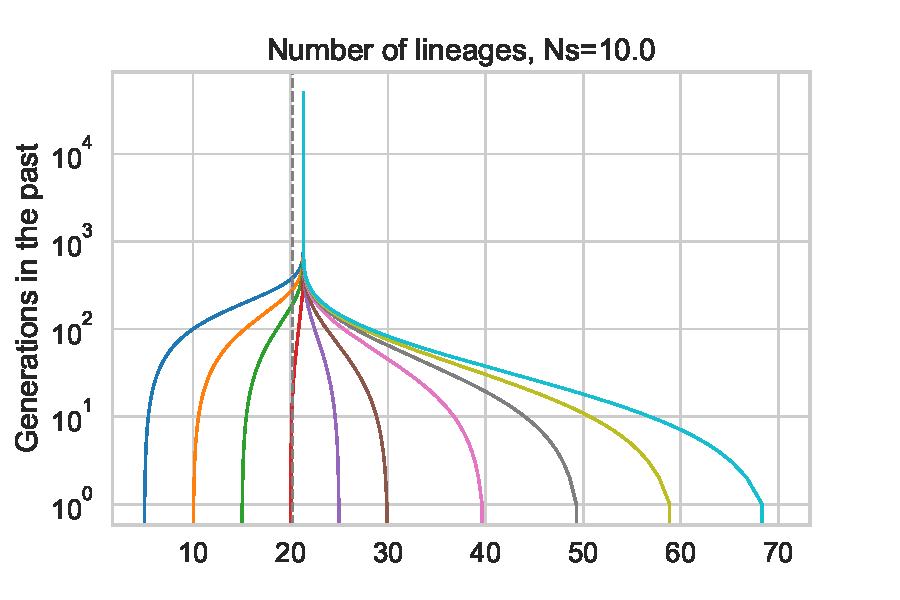
\includegraphics[]{fig/bell-plot.pdf}
  \caption{Expected number of contributing parental lineages back in time. Starting at a given
    sample size, the number of contributions is tracked with align \ref{eq:contributors-back}.
    The $Y$ axis shows time on a logarithmic scale, $X$ axis is the sample size. $N=1000$, $Ns=10$.}
  \label{fig:bell-plot}
\end{figure}


\subsection{Distribution}
\label{subsec:distribution}

We now construct a probability distribution of the number of contributing lineages one generation
into the past.

The number of parental lineages used by drift can be modelled by the modified occupancy
(Arfwedson) distribution \cite{Wakeley2009,ONeill2019,JohnsonEtAl2005}. This is given by:

\begin{align}
  \label{eq:occupancy}
  P(\mathcal{P}=p|\mathcal{G}=g) = \frac{S_2(g,p) N!}{(N-p)! N^g}
\end{align}

where $S_2(g,p)$ is a Stirling number of the second kind, which is the number of ways to partition
$g$ objects into $p$ categories. A typical statement of the occupancy distribution is that we have
$N$ urns and $g$ colored balls, and we want to know the probability that exactly $p$ of the urns
will be occupied (see \cite{JohnsonEtAl2005} section 10.4 for a thorough treatment). In our case,
$N$ is the population size, urns correspond to the parents, colored balls to gametes. Note that the
under drift, the number of parents will be smaller or equal to the number of gametes $p \le g$.

The occupancy distribution is not simple to evaluate, but good performance can be achieved by
pre-computing a table of reduced occupancy numbers, using the algorithm of \cite{ONeill2019}.

As stated before, the number of lineages sampled under selection is described with a negative
binomial distribution. Unlike \ref{eq:neg-binom-fail}, however, we are looking for the total number of
lineages sampled, not simply the number of failed trials. In this parameterization, the probability
of the negative binomial is given by:

\begin{align}
  \label{eq:neg-binomial-trials}
  P(\mathcal{G}=g|n) = \binom{g-1}{n-1}(1-xs)^n(xs)^{g-n}
\end{align}

Here, the number of gametes can be larger that the sample size $n \le g$, if selection is present
($s<0$).

Combining the two distributions together through \ref{eq:conditional}, we get:

\begin{align}
  \label{eq:lineages-in-past}
   Pr(\mathcal{P}=p|n) = \sum_{g=1}^{\infty} \frac{S_2(g,p) N!}{(N-p)! N^g} \binom{g-1}{n-1}(1-xs)^n(xs)^{g-n}
\end{align}

Unfortunately, this distribution does not have a simple analytical form. In certain parameter
regimes, this can be approximated by the normal distribution \cite{JohnsonEtAl2005,ONeill2019},
which we describe in the next section.

Figure \ref{fig:sampling-dist} shows the distribution of the number of contributing parental
lineages for several selection coefficients for a sample $n=20$. In the absence of selection, the
distribution has zero probability above $n=20$, as no extra lineages can be sampled. As the strength
of selection is increased, we begin requiring larger number of lineages. At the equilibrium point
($Ns=10$, \eqref{eq:critical-sample}), the distribution is symmetric.

\begin{figure}
  \centering
  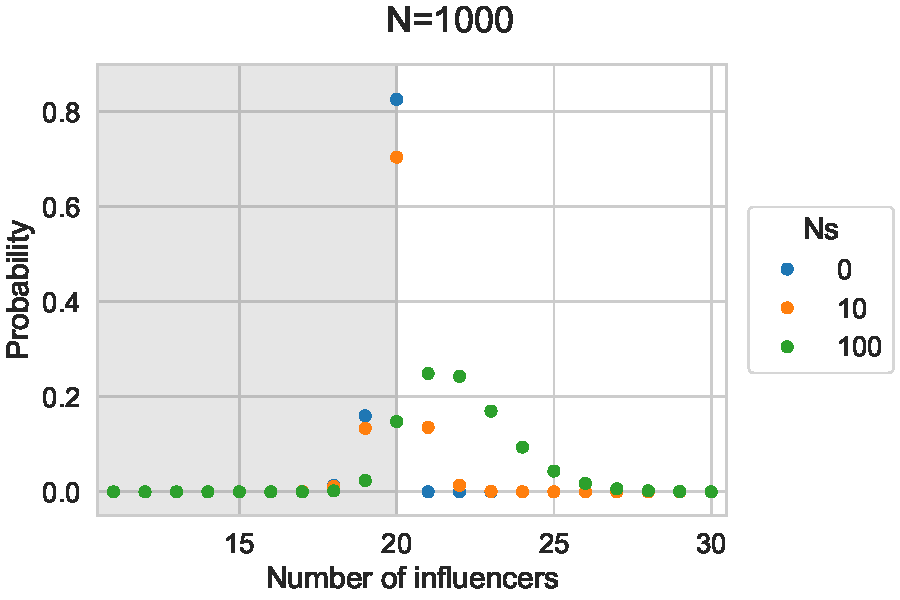
\includegraphics[]{fig/sampling-dist.pdf}
  \caption{The distribution of the number of parental contributing lineages one generation into the
    past ($n=20$, $N=1000$). Shaded area shows the drift-dominated regime, where the number of
    lineages is smaller than the sample size.}
  \label{fig:sampling-dist}
\end{figure}

We note that at the critical sample size, the probability that we will have a sufficient number of
lineages is only $50\%$. In order to guarantee that drift will out-pace selection, we can calculate
the cumulative distribution - Figure \ref{fig:cumulative-dist}. This shows that a sample size in
which the majority of lineages are accounted for can be substantially larger than the critical
sample size of equation \eqref{eq:critical-sample}. To derive a convenient expression, we turn to
the normal approximation in the next section.

\begin{figure}
  \centering
  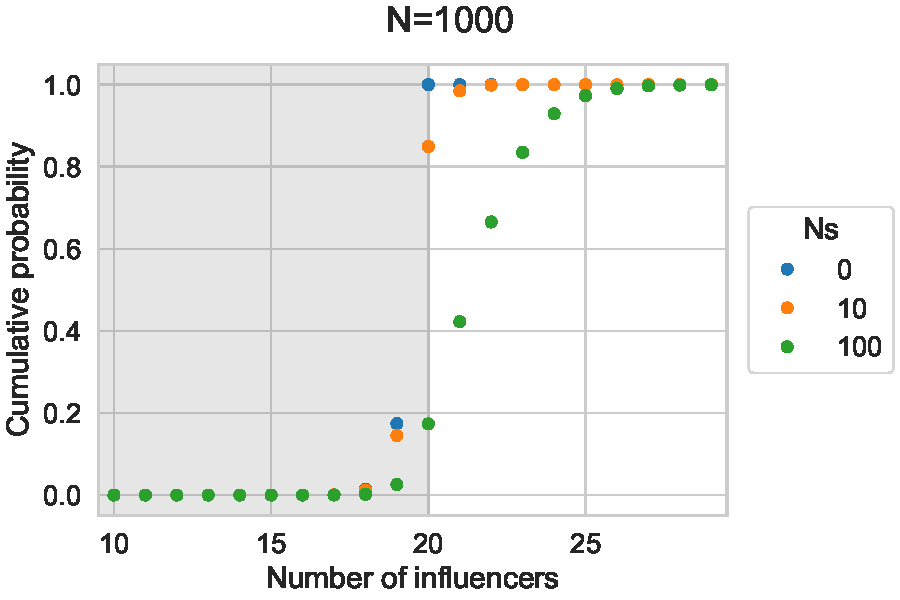
\includegraphics[]{fig/cumulative-dist.pdf}
   \caption{The cumulative distribution of the number of parental contributing lineages one generation into the
    past ($n=20$, $N=1000$). Shaded area shows the drift-dominated regime, where the number of
    lineages is smaller than the sample size.}
  \label{fig:cumulative-dist}
\end{figure}

\subsection{Normal approximation}

Finally, we can construct a normal approximation to the distribution of the number of contributing
lineages. The occupancy distribution is approximated by the normal \cite{ONeill2019} when $n \ll N$.
Likewise, the number of failures (eq. \eqref{eq:neg-binom-fail}) before a given number of successes,
can be approximated by the normal distribution. In the case of large population size, as required by
the approximation of the occupancy by the normal, we can approximate the total number of
contributing lineages as the sum of lineages contributed by the two distributions. The random
variable which is a sum of two normally-distributed random variables is also normal, with
$\mu=\mu_1+\mu_2$ and $\sigma^2 = \sigma^2_1 + \sigma^2_2$. By combining the required expectations
and variance, we find that the normal approximation then has the form:

\begin{align}
  Pr(\mathcal{P}=p|n) \approx \mathcal{N}( \mu &= (s n)/(1 - s) + N (1 - (1 - 1/N)^n),\\
  \sigma &= \sqrt{N \left((N-1) \left(1-\frac{2}{N}\right)^n+\left(1-\frac{1}{N}\right)^n-N\left(1-\frac{1}{N}\right)^{2 n}\right)+\frac{n s}{(1-s)^2}})
\end{align}

Figure \ref{fig:normal-approximation} shows the quantiles of the normal approximation. We see that
up to $99\%$ of the lineages will be contained within the sample of 200 with $Ns=20$. Larger
percentiles will require larger sample sizes.

\begin{figure}
  \centering
  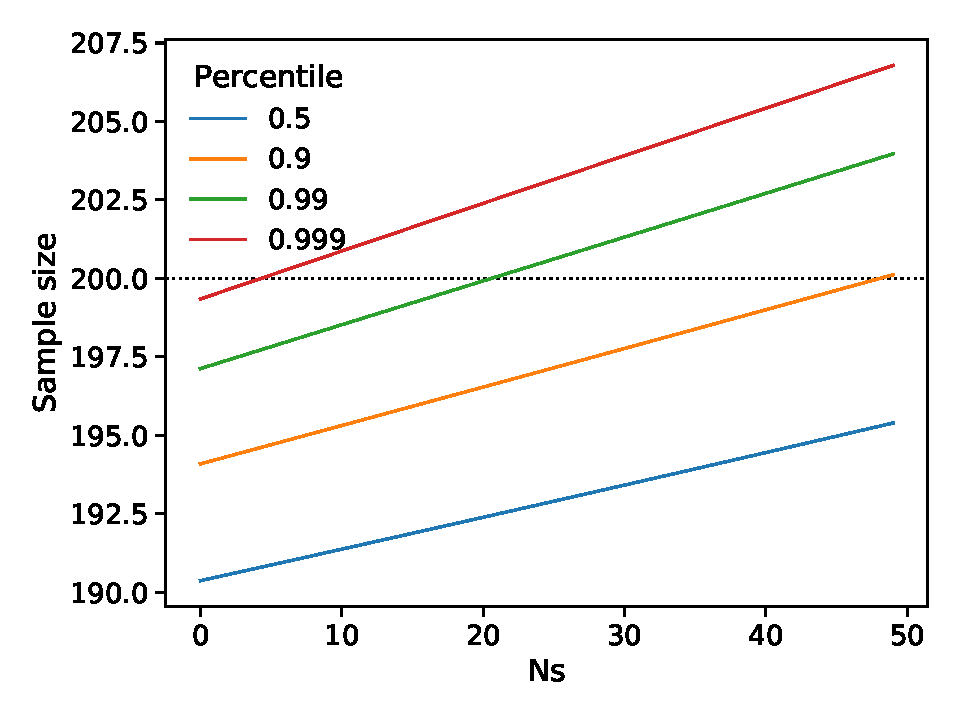
\includegraphics[]{fig/quantile.pdf}
   \caption{The quantile function of the closure of the sample. Each line corresponds to different
     percentile of the normal approximation. Black dashed line shows the reference sample size $n=200$.}
  \label{fig:normal-approximation}
\end{figure}


\section{Conclusion}
\label{sec:conclusion}

In this work we show that with the increasing sample size, the effect of drift overcomes the effect
of selection. As a result, it is possible to construct asymptotically closed solutions to coalescent
with selection, provided the sample size is sufficiently large.

The sample size where the expected number of extra lineages required by selection is less than the
sample size is well approximated by $2Nxs$. However, the sample size that guarantees that almost no
extra lineages are required is considerably larger (\ref{fig:cumulative-dist}).

Using this observation, we can construct a Markov model that describes the number of derived alleles
in the sample. With a sufficiently large sample size, such Markov chains are closed, and can be used
for the calculation of the allele frequency spectra with strong selection.

As a future direction, we want to combine the jackknife approximation \cite{JouganousEtAl2017} with the
results presented here. Since the jackknife is an uncontrolled approximation, the current results
provide a more sensible approach. However, we can still employ the jackknife in the cases where
extra lineages are still required in the current approach. This has the potential of further
improving the accuracy of the model and computational efficiency.


\bibliography{disco}

\end{document}
